\documentclass[dtu]{dtuarticle}
\usepackage{parskip} % use enters instead of indents

\newcommand{\todo}[1]{\color{red}[TODO: #1]\color{black}}
\newcommand*\chem[1]{\ensuremath{\mathrm{#1}}}
\usepackage{amsmath}
\usepackage{bm} % bold ITALIC math (for vectors!)
\usepackage{siunitx}
\usepackage{subcaption}

\title{Machine Learning Project 1}
\subtitle{Data: Feature extraction, and visualization}
\author{Group 94}
\course{02452 Machine Learning}
\address{
	DTU Compute \\
	Fall 2025
}
\date{\today}


\begin{document}

	\maketitle

%	\begin{table}[h!]
%		\renewcommand{\arraystretch}{1.1} % make the spacing a bit nicer
%		\centering
%		\begin{tabular}{l | l}
%			\textbf{Name}                 & \textbf{Student number} \\ \hline\hline
%			Vincent Van Schependom        & s251739                 \\ \hline
%			Diego Armando Mijares Ledezma & s251777                 \\ \hline
%			Albert Joe Jensen             & s204601
%		\end{tabular}
%		\caption{Group members.}
%		\label{table:members}
%	\end{table}
%
%	\begin{table}[h!]
%		\renewcommand{\arraystretch}{1.1} % make the spacing a bit nicer
%		\centering
%		\begin{tabular}{l | *{3}{|l}}
%			\textbf{Task} & \textbf{Vincent} & \textbf{Diego} & \textbf{Albert} \\ \hline\hline
%			Section 1     & 30\%             & 30\%           & 40\%            \\ \hline
%			Section 2     & 40\%             & 30\%           & 30\%            \\ \hline
%			Section 3     & 30\%             & 40\%           & 30\%            \\ \hline
%			Section 4     & 30\%             & 30\%           & 40\%			\\ \hline
%			\LaTeX        & 90\%             & 5\%           & 5\%
%		\end{tabular}
%		\caption{Contributions \& responsabilities table.}
%		\label{table:contributions}
%	\end{table}

	\begin{table}[h!]
		\begin{subtable}{.58\textwidth}
			\begin{tabular}{l | l}
				\textbf{Name}                 & \textbf{Student number} \\ \hline\hline
				Vincent Van Schependom        & s251739                 \\ \hline
				Diego Armando Mijares Ledezma & s251777                 \\ \hline
				Albert Joe Jensen             & s204601
			\end{tabular}
			\caption{Group members.}
			\label{table:members}
		\end{subtable}
		\begin{subtable}{.4\textwidth}
			\begin{tabular}{l | *{3}{|l}}
				\textbf{Task} & \textbf{Vincent} & \textbf{Diego} & \textbf{Albert} \\ \hline\hline
				Section 1     & 30\%             & 30\%           & 40\%            \\ \hline
				Section 2     & 40\%             & 30\%           & 30\%            \\ \hline
				Section 3     & 30\%             & 40\%           & 30\%            \\ \hline
				Section 4     & 70\%             & 15\%           & 15\%			\\ \hline
				\LaTeX        & 90\%             & 5\%           & 5\%
			\end{tabular}
			\caption{Contributions \& responsabilities table.}
			\label{table:contributions}
		\end{subtable}
		\caption{Group information \& work distribution.}
	\end{table}

	\section*{Introduction}

	The objective of this report is to apply the methods that were discussed during the first
	section of the course \textit{Machine Learning} \cite{book} to a chosen dataset. The aim is to get
	a basic understanding of the data prior to the further analysis (project report 2).

	The particular dataset that is being investigated is the \textit{Glass Identification} dataset from 1987 by B. German \cite{dataset}. Table \ref{table:members} lists our full names and student numbers, while Table \ref{table:contributions} shows an overview of the contribution of each team member.

	\tableofcontents

	\newpage

	\section{The \textit{Glass Identification} dataset}

	\todo{The introduction to the data set.}

	\section{A close look at the different attributes}

	\begin{table}
		\centering
		%\renewcommand{\arraystretch}{1.3} % make the spacing a bit nicer
		\begin{tabular}{l|l|l}
			\textbf{Attribute} & \textbf{Description}                    & \textbf{Type of variable} \\ \hline \hline
			\texttt{ID}        & Observation ID (excluded from analysis) & Numeric (discrete)        \\ \hline
			\texttt{RI}        & Refractive Index                        & Continuous                \\ \hline
			\texttt{Na}        & Sodium oxide ($\chem{Na_2 O}$)          & Continuous                \\ \hline
			\texttt{Mg}        & Magnesium oxide ($\chem{Mg O}$)         & Continuous                \\ \hline
			\texttt{Al}        & Aluminum oxide ($\chem{Al_2 O_3}$)      & Continuous                \\ \hline
			\texttt{Si}        & Silicon oxide ($\chem{Si O_2}$)         & Continuous                \\ \hline
			\texttt{K}         & Potassium oxide ($\chem{K_2 O}$)        & Continuous                \\ \hline
			\texttt{Ca}        & Calcium oxide ($\chem{Ca O }$)          & Continuous                \\ \hline
			\texttt{Ba}        & Barium oxide ($\chem{Ba O}$)            & Continuous                \\ \hline
			\texttt{Fe}        & Iron oxide ($\chem{Fe_2 O_3}$)          & Continuous                \\ \hline
			\texttt{type}      & Type of glass                           & Nominal                   \\
		\end{tabular}
		\caption{\todo{Fill in.}}
		\label{table:attributes}
	\end{table}

	\begin{table}
		\centering
		%\renewcommand{\arraystretch}{1.3} % make the spacing a bit nicer
		\begin{tabular}{r|l|l}
			\textbf{} & \textbf{Abbreviation in dataset} & \textbf{Description}                 \\ \hline\hline
			        1 & \texttt{BW-FP}                   & Building Window, Float Processed     \\ \hline
			        2 & \texttt{BW-NFP}                  & Building Window, Non Float Processed \\ \hline
			        3 & \texttt{VW-FP}                   & Vehicle Window, Float Processed      \\ \hline
			        4 & \texttt{VW-NFP}                  & Vehicle Window, Non Float Processed  \\ \hline
			        5 & \texttt{containers}              & Containers                           \\ \hline
			        6 & \texttt{tableware}               & Tableware (e.g. \dots)               \\ \hline
			        7 & \texttt{headlamps}               & Headlamps (e.g. \dots)
		\end{tabular}
		\caption{\todo{Fill in.}}
		\label{table:types}
	\end{table}

	\todo{Detailed explaination of the attributes of the data.}

	\section{Descriptive analysis of the dataset}

	\todo{...}

	\subsection{Extreme values and outliers}

	\textbf{Note that the IQR `rule' is not a ground truth, but rather a way to detect \textit{possible} outliers.}

	\todo{...}

	\subsection{Distribution of the attributes}
	\label{section:distribution}

	\textbf{Note that there are no non-float processed vehicle windows! (\#\texttt{VW-NFP}=0)}

	\todo{...}

	\begin{table}[h!]
		\begin{subtable}{0.6\textwidth}
			\begin{tabular}{r | *{6}{| r}}
				            & \textbf{Mean} & \textbf{Std.} & \textbf{Min} & \textbf{Max} & \textbf{Skew} & \textbf{Kurtosis} \\ \hline\hline
				\texttt{RI} &               &               &              &              &               &                   \\ \hline
				\texttt{Na} &               &               &              &              &               &                   \\ \hline
				\texttt{Mg} &               &               &              &              &               &                   \\ \hline
				\texttt{Al} &               &               &              &              &               &                   \\ \hline
				\texttt{Si} &               &               &              &              &               &                   \\ \hline
				 \texttt{K} &               &               &              &              &               &                   \\ \hline
				\texttt{Ca} &               &               &              &              &               &                   \\ \hline
				\texttt{Ba} &               &               &              &              &               &                   \\ \hline
				\texttt{Fe} &               &               &              &              &               &
			\end{tabular}
			\caption{Summary statistics.}
			\label{table:summary-stats}
		\end{subtable}
		\hspace*{0\textwidth}
		\begin{subtable}{.3\textwidth}
			\begin{tabular}{r|l|l|l}
				  & \texttt{type}       & \textbf{Cnt.} & \textbf{Freq.} \\ \hline\hline
				1 & \texttt{BW-FP}      &                &                \\ \hline
				2 & \texttt{BW-NFP}     &                &                \\ \hline
				3 & \texttt{VW-FP}      &                &                \\ \hline
				4 & \texttt{VW-NFP}     &                &                \\ \hline
				5 & \texttt{containers} &                &                \\ \hline
				6 & \texttt{tableware}  &                &                \\ \hline
				7 & \texttt{headlamps}  &                &
			\end{tabular}
			\caption{Absolute and relative frequencies of \texttt{type}.}
			\label{table:frequencies}
		\end{subtable}
		\caption{\todo{Fill in.}}
	\end{table}

	\subsection{Correlation between attributes}

	\todo{...}

	\section{Principal Component Analysis}

	\todo{Explain why we standardise.}

	Because the attributes are on completely different scales (Section \ref{section:distribution}), we standardise the variables by subtracting their mean and subsequently dividing by the standard deviation.

	\subsection{Dimension reduction}

	We aim to reduce the 9-dimensional dataset into an $M$-dimensional one (with $M < 9$).

	\todo{How many PC's do we keep? I think $M=5$.}

	\subsection{Principal directions}

	The \textit{principal directions} of the (first $M$) principal components are the rotations, corresponding to each principal component $\text{PC}_i = \bm{v_i}$ in the transform-matrix $\bm{V}_M$. This matrix is used when computing the projected coordinates $\bm{B} = \bm{V}_M \bm{X}$ of the original data $\bm{X}$ onto the subspace spanned by the first $M$ principal components.

	\begin{table}[h!]
		\centering
		\begin{tabular}{r | *{3}{|r}}
			\textbf{Variable} & $\textbf{PC}_1$ & ... & $\textbf{PC}_M = \textbf{PC}_{5??}$ \\ \hline \hline
			\texttt{RI} & \num{0} & ... & \num{0} \\
			\texttt{Na} & \num{0} & ... & \num{0} \\
			\texttt{Mg} & \num{0} & ... & \num{0} \\
			\texttt{Al} & \num{0} & ... & \num{0} \\
			\texttt{Si} & \num{0} & ... & \num{0} \\
			\texttt{K} & \num{0} & ... & \num{0} \\
			\texttt{Ca} & \num{0} & ... & \num{0} \\
			\texttt{Ba} & \num{0} & ... & \num{0} \\
			\texttt{Fe} & \num{0} & ... & \num{0}
		\end{tabular}
		\caption{The principal directions (a.k.a. the \textit{loadings}) of the first $M$ principal components $\text{PC}_i = \bm{v_i}$ in the rotation matrix $\bm{V}_M$. \todo{Describe what these directions mean in terms of the original attributes.}}
		\label{table:loadings}
	\end{table}

<<<<<<< Updated upstream
	\subsection{Projected data}

	\todo{Visualisations of the projected data}
=======
	\begin{figure}
		\centering
		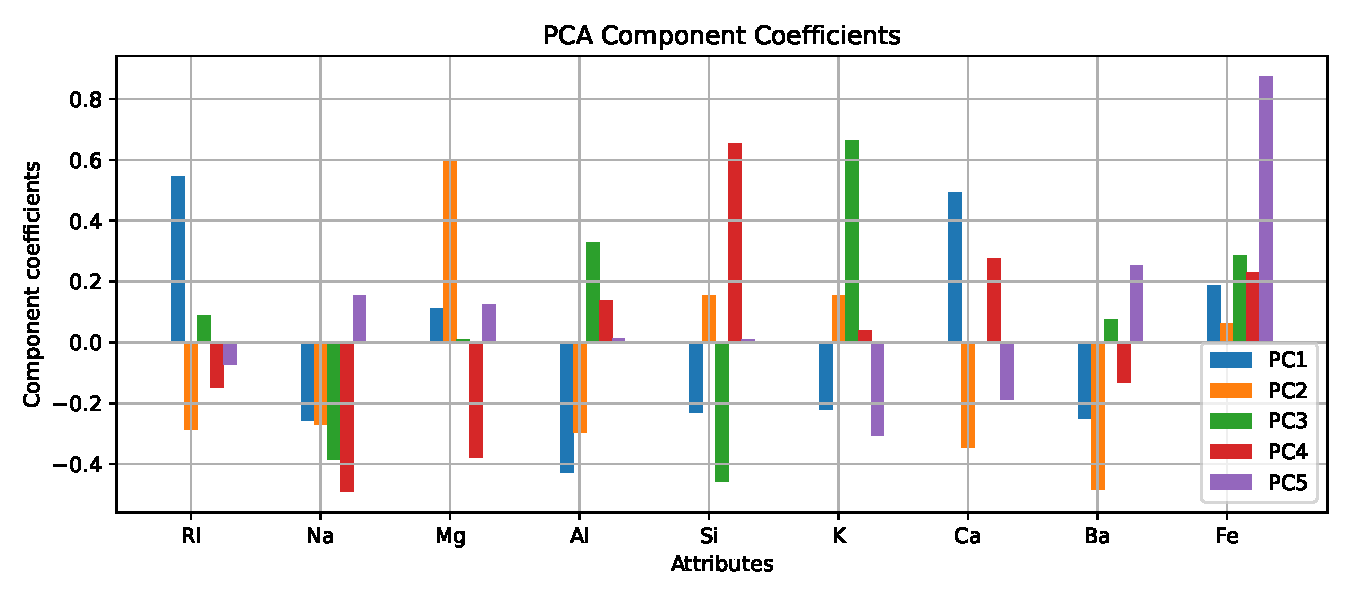
\includegraphics[width=.99\textwidth]{figures/pca_component_coefficients}
		\caption{Loadings of the original variables on the first five principal components. Positive and negativ values indicate the \textit{direction} of influence, while the magnitude reflects the \textit{strength} of the contribution.}
		\label{fig:pc-components}
	\end{figure}

	Based on the loadings in Table \ref{table:loadings} and the corresponding visualisation in Figure \ref{fig:pc-components}, the first principal component ($\text{PC}_0$) is most strongly influenced by \texttt{RI} and \texttt{Ca}, which carry positive loadings, and negatively by \texttt{Al} and \texttt{Si}. This suggests that $\text{PC}_0$ captures a trade-off between refractive index and calcium content versus aluminium and silicon.

%	Shortened version of the stuff that is beneath this comment:
%	The second principal component ($\text{PC}_1$) places strong weight on \texttt{Mg} and negative weight on \texttt{Ba}, indicating a contrast between magnesium and barium content. Later components highlight more specific variations, such as $\text{PC}_4$, which is dominated by \texttt{Fe}, pointing to a component that largely isolates variation in iron concentration.

	\todo{Check all loadings and the text below.}

	The second principal component ($\text{PC}_1$) assigns a large positive loading to \texttt{Mg}, while strongly down-weighting \texttt{Ba} and, to a lesser degree, \texttt{Na}. This indicates that $\text{PC}_1$ primarily reflects a contrast between magnesium concentration and the presence of barium and sodium.

	The third principal component ($\text{PC}_2$) is dominated by a large positive loading for \texttt{K}, balanced by strong negative contributions from \texttt{Si} and \texttt{Na}. This points to a dimension that separates potassium-rich compositions from those with higher silica and sodium content.

	The fourth principal component ($\text{PC}_3$) shows high positive contributions from \texttt{Si}, \texttt{Ca}, and \texttt{Fe}, with negative influence from \texttt{Mg} and \texttt{Na}. It therefore captures variation where higher levels of silicon, calcium, and iron occur together in opposition to magnesium and sodium.

	Finally, the fifth principal component ($\text{PC}_4$) is characterised by a dominant positive loading for \texttt{Fe}, while moderately influenced by \texttt{Ba} and negatively by \texttt{K}. This indicates that $\text{PC}_4$ primarily isolates variation in iron concentration, with some contribution from the balance between barium and potassium.

	\subsection{Projected data}

	\subsubsection{Biplots}

	The projection of the standardised dataset onto the principal component axes produces a lower-dimensional representation that can be visualised in two-dimensional \textit{biplots}. In these plots:

	\begin{itemize}
		\item Each point corresponds to a \textit{score}, representing the coordinates of an original observation in the space spanned by the selected principal components. The scores have been \textit{rescaled} to the interval $[-1,1]$ to facilitate comparison with the arrows, representing variable loadings.
		\item The arrows correspond to the \textit{loadings}, i.e., the contributions of the original variables to the principal components. The direction of an arrow indicates how the variable influences the component axes, and its length reflects the magnitude of this influence.
	\end{itemize}

	Together, scores and loadings allow for simultaneous interpretation of both the observations and the variables.

	\subsubsection{Interpretation based on glass types}

	Figure~\ref{fig:biplots} shows two biplot visualisations. In the first biplot (PC1 vs.\ PC2), which captures \SI{50}{\percent} of the variance, the dominant trends in the data are visible, and some separation between glass types can be observed \todo{explain}. For the second biplot, \todo{fill out.}

	\todo{Make the text below more specific (this is just general GPT-generated stuff)}

	The projected scores reveal that some classes, such as \texttt{BW-FP} and \texttt{R}, cluster distinctly in the reduced space, whereas others, such as \texttt{LW-FP} and \texttt{GL}, exhibit more overlap. The loadings indicate that the separation of classes along the axes is largely driven by specific chemical compositions; for example, PC1 contrasts samples with high \texttt{RI} and \texttt{Ca} against those with higher \texttt{Al} and \texttt{Si}, explaining why some classes separate along this component. \todo{Explain the concrete projections of the different classes further.}

	\begin{figure}[h!]
		\centering
		\begin{subfigure}{0.49\textwidth}
			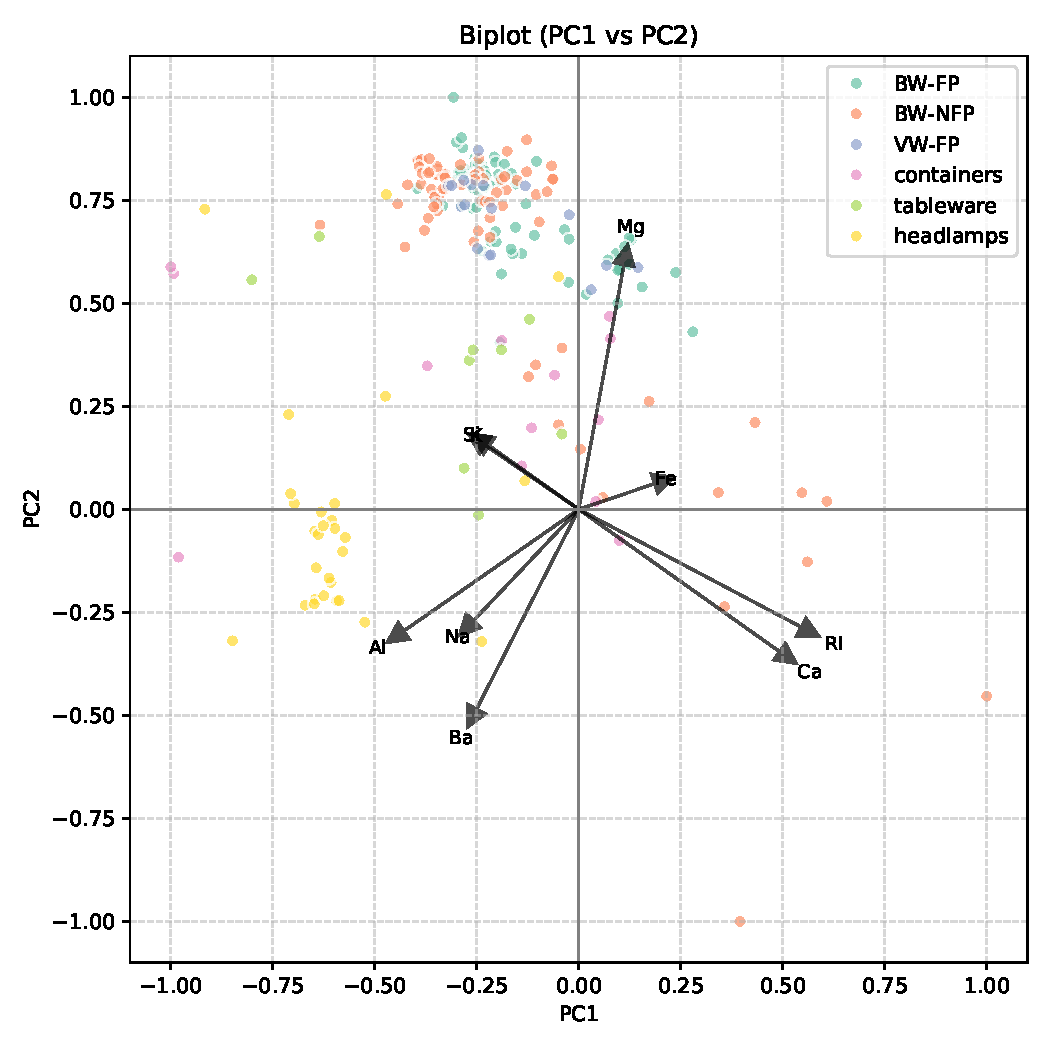
\includegraphics[width=\linewidth]{figures/pca_biplot_pc1_pc2.pdf}
			\caption{PC1 vs PC2}
			\label{fig:biplot_pc1_pc2}
		\end{subfigure}
		\hfill
		\begin{subfigure}{0.49\textwidth}
			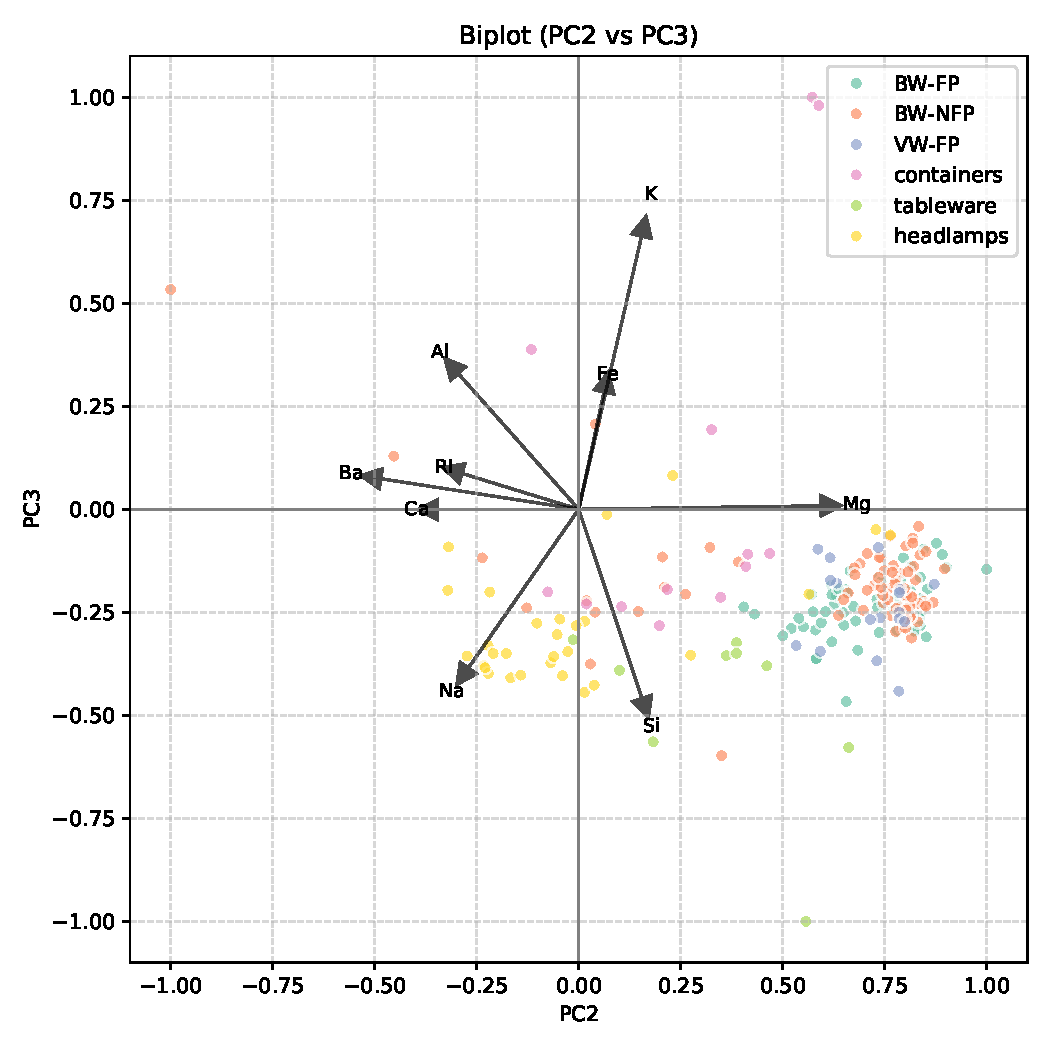
\includegraphics[width=\linewidth]{figures/pca_biplot_pc2_pc3.pdf}
			\caption{PC2 vs PC3}
			\label{fig:biplot_pc1_pc3}
		\end{subfigure}
		\caption{Biplots of the glass dataset showing both projected samples (colored by class) and variable loadings.}
		\label{fig:biplots}
	\end{figure}

	\subsubsection{Extreme scores}

	\todo{Explain the observations that score extremely high/low in certain principal directions.}

	\section{Use of GenAI}

	\todo{Explain what kind of GenAI you used.}
>>>>>>> Stashed changes

	\section*{Summary}

	\todo{A short summary of what we discussed in the whole paper.}

	\bibliography{citations}
	\bibliographystyle{unsrt}

\end{document}
